\section{Durchführung}
\label{sec:Durchführung}

Der Versuchsaufbau ist in Abbildung \ref{fig:bild2} dargestellt.

\begin{figure}[H]
    \centering
    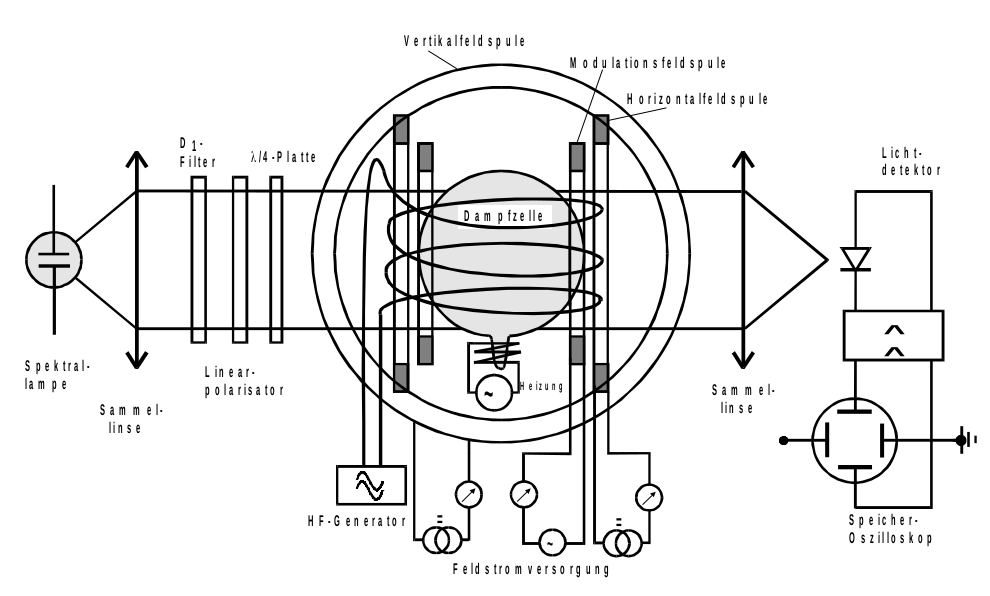
\includegraphics[scale=0.4]{content/bild2.png}
    \caption{Versuchsaufbau zum Vorgang des optischen Pumpens mit rechtszirkular polarisiertem Licht [2]}
    \label{fig:bild2}
  \end{figure}

Das Licht einer Rubidium-Spektrallampe wird durch einen Frequenzfilter, einen Linearpolarisator und eine $\frac{\lambda}{4}$-Platte
bezüglch seiner Frequenz gefiltert und rechtszirkular polarisiert und trifft dann auf die mit Rubidium  $\ce{^{85}Rb}$
und  $\ce{^{87}Rb}$ gefüllte Dampfzelle, die durch eine Heizspirale beheizt wird und von vier Spulen umgeben ist.
Die vertikal angeordnete Spule dient zum Ausgleich des Erdmagnetfeldes, die horizontal ausgerichteten zur Modulation des
Magnetfeldes und die an den Hochfrequenzgenerator angeschlossene zur Anregung.
Hinter der Dampfzelle wird das transmittierte Licht gemessen und das Signal an ein Oszilloskop übergeben.

Das Rubidium wird durch die Heizspirale erhitzt, sodass idealer Dampfdruck vorhanden ist. Die optischen Elemente, insbesondere
die abbildenden Linsen, werden justiert. Zudem wird die Horizontalkomponente des Erdmagnetfeldes durch Ausrichtung
des Versuchsaufbaus in Nord-Süd-Richtung und die Vertikalkomponente durch die Vertikalspule  ohne angelegtes
Modulationsfeld so gut wie möglich ausgeglichen.
Modulationsspule und Messdiode werden an das Oszilloskop im XY-Modus angeschlossen.
Es werden die Modulationsmagnetfelder der Minima für Hochfrequenzen von $\num{100}$ bis $\SI{1000}{\kilo\hertz}$
gemessen. Der Modulationsbereich kann mithilfe der Horizontalspule verschoben werden.


